\documentclass[10pt]{article}
\usepackage[margin=1in]{geometry}
\twocolumn
%\usepackage{stfloats} 
\usepackage{graphicx}
\begin{document}
\author{Daniel Speyer\\dls2192@columbia.edu \and Johan Mena\\j.mena@columbia.edu}
\title{A Recursive Systemic Profiler}

\twocolumn[
\begin{@twocolumnfalse}
\maketitle

\end{@twocolumnfalse}
]

\begin{abstract}
The first task in writing any performant code is to understand where it is spending its time. This allows programmers both to apply optimizations where they will make a difference, and to not optimize where it won't make a difference. The standard tools for this are profilers, which measure where processes spend their time while running. However many processes spend most of their total wall time in actions not measured by traditional profilers. Here, we propose and implement a Recursive Systemic Profiler, a tool that can give a more complete view of the causes of an application’s performance in Linux system.

\section{Introduction}
Even though premature optimization is the root of all evil, profiling the performance of a system is critical for its improvement. Profiling is, however, no small task: WHY. As systems become more complex, it is becoming increasingly important to become familiar with several profiling tools that can aid in understanding them. The motivation of the Recursive Systemic Profiler is simple: to show how processes spend their time. This allows programmers and system administrators to answer questions like: Why is this process slow? What is it waiting on? What is the reason it is spending this many resources?

We know from experience that, most of the time, the slowness of systems comes from very specific parts of the codebase (as opposed to the entire system). As programmers, we want to be able to identify where this is so we can optimize that and not waste time optimizing other, unimportant parts.

We present RSP, which blah.
The rest of the paper is organized as follows. Section 2 lays out the background 

\section{Background: Data Collectors}
In order to make sense of the performance of a system, one first need to collect data. There are several open source profiling tools that focus on this task. We can classify them in three different groups by the approach they use to collect information: event-based, sample-based and a combination of both. 

Event-based tools work by instrumenting programs: they insert marks at different points of a system and trigger an event when the profiled application runs into them. These events can trigger simple data-collection actions like incrementing a counter, but they can also perform more complicated tasks like generating stack dumps or generating some kind of logging.

Sample-based tools work by collecting samples of programs at regular intervals.  Samples be performance counters, stack traces, or something else of relevance. These kinds of profilers are typically less accurate than event-based profilers since they rely on , but they since they don't introduce the overhead of generating events, they are usually less intrusive with respect with the profiled application.

A third approach combines event-based and sample-based profiling.

There are a variety of open source tools at our disposal for collecting data within Linux-based operating systems. They vary in functionality and mode of use depending on, for example, the part of the operating system the user is interested in analyzing or the information granularity desired.

Some of the most popular tools include perf for system-wide profiling, strace for system call profiling or netstat for network profiling.

One of the first questions that arises when trying to create a tool like the Recursive Systemic Profiler is: how will it gather its data? Since RSP focuses on giving users a full-picture view of the system, we decided we needed a tool that system-wide reach to gather its data. After evaluating a few of the tools that were available, we determined we should try out three different such tools and decide on one of them: lttng, perf and DTrace.

Since creating a profiler from scratch would have been a daunting task (to say the least), we instead chose to build our tool on top of one of the most widely popular and supported profilers available at the moment: perf.

\subsection{Linux Perf Events}

Linux Perf Events, also known as perf\_events or just perf, compared to other tools like ftrace or lttng, has the advantage of being a mature and actively developed tool that can collect system-wide information in an event-oriented fashion: it is able to tap into hardware events like CPU cycles and memory cache misses; software events like CPU migrations and minor faults; as well as high-level behavior like system calls, TCP events, disk and file system I/O, etc.

One other characteristic we needed in a tool was the confidence that it was  In addition to these characteristics, perf is part of the Linux kernel itself, so not much extra software is needed in order for one to start profiling applications.

\section{Visualizations}
Visualizations are at the heart of the Recursive Systemic Profiler. Not only do visualizations help to understand what's happening in a system in a shorter period of time compared to looking at plain old statistics, but they also show at-a-glance information that can easily be missed when only reading raw numbers. After evaluating several approaches of data visualization for profilers, we felt we needed to emulate something akin to flame graphs.

\subsection{Flame Graphs}
Flame Graphs, a visualization tool invented by Brendan Gregg, are a simple way to visualize stack traces. Stack traces contain the names of the functions being executed by the CPU at any given time. Flame graphs present this information in a hierarchical manner, in such a way that one can easily tell which function called which other function, in a clear, chain-like manner.

Flame graphs also have the characteristic  are able to show at a glance overall hot-spots shows overall program structure


\section{Recursive Systemic Profiler}

The Recursive Systemic Profiler is designed to measure all the activities that contribute to the running time of a program.  It is ``systemic'' in that it records everything that takes place on the system and ``recursive'' in that it starts from a process of interest, then considers processes that was waiting for, and processes those were waiting for, and so on.

The building blocks the profiler works with are runs, sleeps, links and samples.  A run is a contiguous block of time during which a process is running.  A sleep is a similar block in which the process is not running.  A link marks one run causing another.  And a sample is taken by the sampling profiler.  Each sample is part of a run, but very short runs may not have any samples.

\subsection{Scheduling Information}

Linux Perf Events provides annotations for task switches and wakeups, along with stacks.  Task switches are when one process relinquishes a CPU and another takes over (either of the processes may be the idle process).  A stack is given for the departing process.  Wakeups are when a thread becomes marked as runnable (it may not be scheduled for some time).  The Linux kernel is very good at keeping relevant stacks for wakeups.  For example, if a process writes to a TCP socket that connects to localhost, the user function calls write which notices the file handle is a socket and calls send which notices the destination is localhost and calls receive which notices a process is blocked reading from that socket and calls wakeup.  This entire stack is captured intact by perf.

By examining the timing and stacks of these events, we are able to divide task-switches into categories:

\subsection{Interrupts}

Sometimes a process switches out because the CPU it's on has received an interrupt.  Linux uses very small interrupt handlers which pass tasks to high-priority worker threads, rather than do significant work inside the interrupt handler.  This includes cases where a process is pre-empted because it has exhausted its CPU allocation, which we can think of as ``handling a timer interrupt,'' though that is quite rare in practice.

\subsection{Transfers vs Forks}

For non-interrupts, one process wakes another up and then goes to sleep itself.  In this case, we say that one process has ``transfered'' control to another.  When it does not, we say that the thread of control has ``forked''.

\subsection{Pseudo-stacks and Control Paths}

A set of runs connected only by transfer links can be called a ``control path''.

One common pattern is for one process to transfer control to another, and then the other to transfer control back.  Both transfers could be tcp messages, as in the case of making a synchronous rpc request to a database, or one could be a \begin{tt}fork\end{tt} syscall and the other a \begin{tt}wait\end{tt} syscall terminated by the other's exit.  In these cases, it is fairly reasonable to think of the first transfer as a ``function call'' and the second as a ``return''.

While not every pattern of process interaction naturally fits this view, those which don't can generally be shoehorned to fit with fairly little damage.  For example, if one process wakes another which wakes a third which wakes the original, we can think of the first as having been a child of the second, even thought the call went directly.

Once we have this concept of calls and returns, we can assemble the processes into something like a stack.  Note that only the top element of the stack will be a run -- all the rest will be sleeps.

\subsection{Views}

Once we have our data gathered, the next task is to visualize it.  We have several views to do this with.

Our examples here use a toy program called ``pass''.  Pass forks two processes, connects them with pipes, and then runs in a loop in which one process does some work, then writes to one pipe (waking the other process) and reads from the other pipe (blocking on the other process).  It is called ``pass'' because it passes the act of doing work back and forth.

\subsubsection{Process Running View}

The first view is the Process Running View.  It uses an x axis of time and a y axis of processes.  Each run is a block bar, and each link is drawn as a line between them.  The line is red for a transfer, or blue for a fork.

\begin{figure}[h]
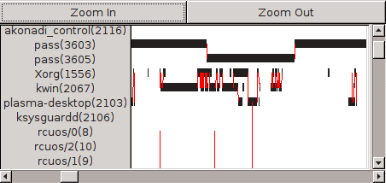
\includegraphics[width=3.25in]{screenshot}
\caption{The Process Running View}
\end{figure}

The view also contains an option to show sleeps, which are drawn as blue boxes.  Sleeps are labeled with one function from the stack which best describes the sleep.  At the moment, this is the innermost userspace function, which roughly corresponds to the blocking syscall as the programmer would conceive of it.

Clicking on a process name opens a Flame View for that process.

\subsubsection{Flame View}

The Flame View takes a single process and shows all associated processes, organized into control paths.  Each control path is treated as a series of pseudostacks, and each layer of each pseudostack is drawn as its stack.  This presents the concept of a single stack of functions stretching across multiple processes, which is a pretty good fit for how many programs are actually designed.

\begin{figure}[h]
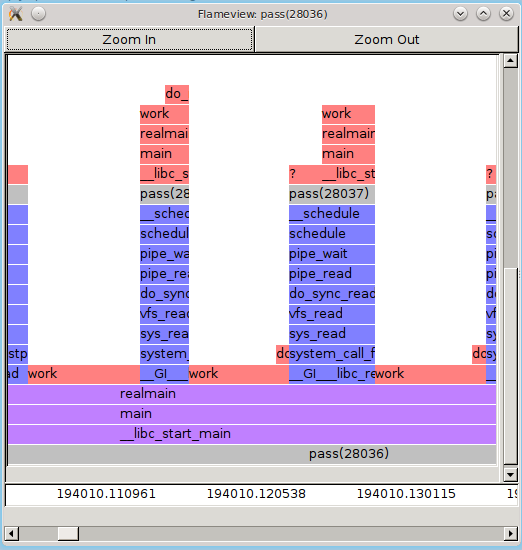
\includegraphics[width=3.25in]{flameshot}
\caption{The Chronological Flame View}
\end{figure}

Functions in a run stack are shown in red, whereas those in a sleep stack are shown in blue.  Process names are shown in grey.  Links are still shown, though links within a control process tend to be largely invisible.

If a run has multiple samples, the horizontal space of the run is divided equally.

The x axis is still time, but now the y axis is stack depth.

\subsection{Implementation}
\subsubsection{Data Collection}

\pretolerance=1000

All data is collected from Linux Perf Events, using the \\ \begin{tt}sched:sched\_wakeup\end{tt}, \begin{tt}sched:sched\_switch\end{tt}, \\ \begin{tt}sched:sched\_process\_exec,\end{tt} and \begin{tt}cycles\end{tt} events.  The data is then dumped in a textual format using the \begin{tt}perf script\end{tt} command.

\pretolerance=200

\subsubsection{Assembling Runs, Sleeps and Links}

The first processing pass simply reads in text and creates a series of event objects.  Each object corresponds to a single event as perf understands the concept.  This pass also attaches stacks to the correct events.

The data is then read into a  state machine that creates runs, sleeps and links.  While passing through, the system keeps track of when each process last started or stopped, what stack each process departed with, and what links are still being assembled.  Links have three timestamps attached: when the wakeup event occurred, when the target process started running, and when the source process stopped running.

Links for which the source process stopped less than $100\mu s$ after the wakeup event are regarded as ``transfer'' links.  This number is arbitrary, but seems to work pretty well in practice.

\subsubsection{Working Around Interrupts}

Wakeup events can be identified as interrupts if the departing stack contains either \begin{tt}do\_IRQ\end{tt} or \begin{tt}apic\_timer\_interrupt\end{tt}.  For interrupts, we do not make a link between the processes, but instead make a link between the two runs of the interrupted process that have the interrupt in between them.  This link is marked as ``horizontal'', because it does not correspond to a change of stack layer.

\subsubsection{Recursive Stack Making}

We assemble pseudostacks recursively, going backwards in time.  We start with the process of interest, then look at what woke it and so on.  All wakings are seen as going deeper into the stack unless this would cause a process to appear on the stack twice.  Since a process that is blocked, waiting on the thing it spawned to finish is not listening to other processes, we generally shouldn't one process twice.  There are a few possibilities involving select calls which we will simply accept a suboptimal visualization of, and signals, which are rare.

\subsubsection{Consolidating}
\subsubsection{Visualizing}

All visualizations are drawn using gtk.

\section{Evalutation}
\subsection{squirrelmail}
\subsubsection{Visualization}
\subsubsection{How Much Is Explained}
\subsubsection{Comparisons}
\subsection{Other tests}
\subsubsection{apt-get}
\subsubsection{chrome load}
\end{document}
